%\cref{fig:传输式谐振腔铁磁共振实验光路图}}
\subsubsection{体效应微波振荡器工作曲线及性能} % (fold)
	\label{ssub:体效应微波振荡器工作曲线及性能}
	\par 预热后按\cref{fig:传输式谐振腔铁磁共振实验光路图}连接仪器,按下微波源信号的“等幅"和“教学"工作钮,固定频率为9.000GHz,测得的体效应管在0$\sim$13V区间电流-电压曲线如\cref{subfig:IV,tab:IV},
	可见大致在3.00-4.50V之间有一个负阻区(指二极管的微分电阻$\diff{V}{I}$小于零),
	这一阶段高场畴逐渐形成,电流随电压升高而减小;
	% 8.50-12.50V又有一个负阻区,这是由于总电压更大以后高场畴得以进一步扩大,此过程形成又一个负阻区;
	由此可见微波工作区应在4.50V以上,即令交变电压的最小值仍大于此值,使得一个高场畴被阳极吸收时下一个畴能同时在阴极成核,从而不断地发射电流脉冲,产生微波。
	% 从电流-电压图像来看,微波振荡的产生是因为在直流偏压达到负阻区后,二极管两端电压振荡频率的任何微小变化都将逐渐增大(负阻区内外加电压增大导致总电流减小而促进电压随之减小,电压减小到负阻区下界时电流又随电压上升而上升,促进电压回到负阻区内,从而使振荡幅度自发增大),最终电压振荡区间稳定在略大于负阻区的范围内。
	%分析体效应管的负阻区和微波工作区的电压范围。
	\par 用吸收式波长计和检波器1测得的10$\sim$13V区间内的频率-电压曲线如\cref{subfig:fV,tab:fV}。可见微波二极管输出的频率随着工作电压升高而缓慢减小。这是由于输出频率由高场畴的渡越时间$T_D$决定\supct{bib:pku}:
	\begin{equation}
		f=\dfrac{1}{T_D}=\dfrac{v_D}{L}
	\end{equation}
	而畴的平均速率$v_D$主要是由成熟畴的电荷量决定的,电压越高,高场畴越大,渡越速度越慢,所以
	% 场畴成熟越快,高场畴成熟时的总电量就越小,
	输出频率就越低。
	\begin{figure}[htbp]
		\subfloat[电流-电压变化关系]{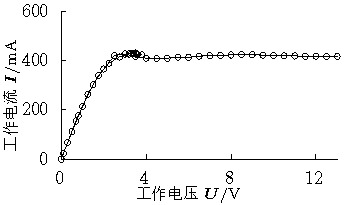
\includegraphics[height=3cm]{dat/prc/IV.pdf}\label{subfig:IV}}\hfill
		\subfloat[频率-电压变化关系]{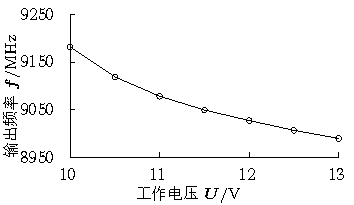
\includegraphics[height=3cm]{dat/prc/fV.pdf}\label{subfig:fV}}\hfill
		\subfloat[输出功率-频率变化关系]{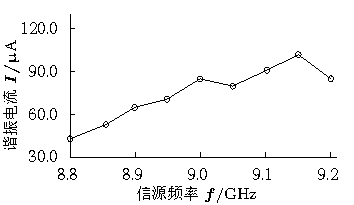
\includegraphics[height=3cm]{dat/prc/If.pdf}\label{subfig:If}}
		\caption{体效应微波振荡器工作特性}
	\end{figure}
	\begin{table}[htbp!]
	\centering\small
	\caption{工作电流-工作电压关系}\label{tab:IV}	\begin{tabular}{c||c|c|c|c|c}
		\hline\hline
		工作电压$U$/V & 工作电流$I$/mA & 工作电压$U$/V & 工作电流$I$/mA & 工作电压$U$/V & 工作电流$I$/mA\\		\hline\hline
		13.00 & 417 & 6.00 & 414 & 0.30 & 68\\		\hline
		12.50 & 417 & 5.50 & 414 & 0.70 & 155\\		\hline
		12.00 & 418 & 5.00 & 410 & 0.80 & 176\\		\hline
		11.50 & 418 & 4.50 & 409 & 1.25 & 263\\		\hline
		11.00 & 419 & 4.00 & 410 & 1.75 & 340\\		\hline
		10.50 & 420 & 3.50 & 417 & 2.25 & 389\\		\hline
		10.00 & 421 & 3.00 & 427 & 2.75 & 415\\		\hline
		9.50 & 422 & 2.50 & 420 & 3.20 & 427\\		\hline
		9.00 & 424 & 2.00 & 366 & 3.30 & 429\\		\hline
		8.50 & 425 & 1.50 & 302 & 3.40 & 430\\		\hline
		8.00 & 423 & 1.00 & 213 & 3.50 & 431\\		\hline
		7.50 & 422 & 0.50 & 112 & 3.52 & 427\\		\hline
		7.00 & 420 & 0.00 & 0 & 3.60 & 424\\		\hline
		6.50 & 418 & 0.10 & 24 & 3.80 & 424\\		\hline\hline
	\end{tabular}
\end{table}
	\begin{table}[htbp!]
	\centering\small
	\caption{输出频率-电压关系}\label{tab:fV}	\begin{tabular}{c||c|c|c|c|c}
		\hline\hline
		工作电压$U$/V & 频率计读数/mm & 输出频率$f$/MHz & 工作电压$U$/V & 频率计读数/mm & 输出频率$f$/MHz\\		\hline\hline
		13.0 & 8.353 & 8990.0 & 11.0 & 7.508 & 9078.5\\		\hline
		12.5 & 8.186 & 9007.0 & 10.5 & 7.149 & 9119.0\\		\hline
		12.0 & 7.992 & 9027.5 & 10.0 & 6.612 & 9182.0\\		\hline\hline
	\end{tabular}
\end{table}
	\begin{table}[htbp!]
	\centering\small
	\caption{谐振电流-频率关系}\label{tab:If}	\begin{tabular}{c||c|c|c|c|c}
		\hline\hline
		信源频率$f$/GHz & 谐振电流$I/\upmu$A & 信源频率$f$/GHz & 谐振电流$I/\upmu$A & 信源频率$f$/GHz & 谐振电流$I/\upmu$A\\		\hline\hline
		9.103 & 91.1 & 9.050 & 80.0 & 8.899 & 65.0\\		\hline
		9.201 & 85.1 & 9.000 & 85.0 & 8.855 & 53.0\\		\hline
		9.151 & 102.0 & 8.949 & 70.8 & 8.800 & 43.0\\		\hline\hline
	\end{tabular}
\end{table}
	\par 弹起“教学"工作钮后体效应管工作固定在标准电压12.0V左右。在8.9GHz-9.2GHz范围内调节输出频率,调谐检波器1测得的微波输出功率的变化情况如\cref{subfig:If,tab:If}。这是此晶体管本身的工作特性。
% subsubsection 体效应微波振荡器工作曲线及性能 (end)
\subsubsection{铁磁共振实验} % (fold)
	\label{ssub:铁磁共振实验}
	\par 本实验中传输式谐振腔采用TE$_{10p}$矩型谐振腔(本实验中$p$=8, $a$=2.295cm,$l$=19.30cm),故理论上谐振频率为(据\cref{eq:beta}):
	\begin{equation}
		f_0=\dfrac{c\sqrt{p^2+l^2/a^2}}{2l}=9.014\times 10^9{\rm Hz}.
	\end{equation}
	实测谐振频率约为9.026GHz,与计算结果相近。
	\par 在此频率左右连续调节微波频率,用共振仪测出检波示数,即传输式谐振腔的功率指示电流随微波频率的变化关系如\cref{fig:铁磁共振图象,tab:I2f}所示。
	\begin{table}[htbp!]
	\centering
	\caption{谐振电流-频率关系}\label{tab:I2f}	\begin{tabular}{c||c|c|c}
		\hline\hline
		信源频率$f$/GHz & 检波2电流$I$/A & 信源频率$f$/GHz & 检波2电流$I$/A\\		\hline\hline
		9.000 & 2.4 & 9.026 & 65.9\\		\hline
		9.008 & 2.3 & 9.028 & 28.8\\		\hline
		9.015 & 2.3 & 9.029 & 11.0\\		\hline
		9.022 & 5.9 & 9.030 & 7.0\\		\hline
		9.023 & 11.1 & 9.034 & 3.2\\		\hline
		9.025 & 54.0 & 9.039 & 2.3\\		\hline
		9.026 & 88.0 & 9.045 & 2.3\\		\hline\hline
	\end{tabular}
\end{table}
	\FloatBarrier
	\begin{wrapfigure}[]{r}[0pt]{7cm}
		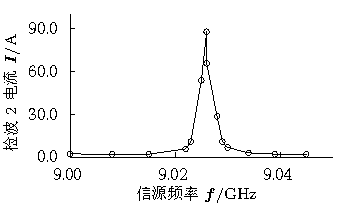
\includegraphics[width=6cm]{dat/prc/I2f.pdf}\caption{铁磁共振图象\label{fig:铁磁共振图象}}
	\end{wrapfigure}
	\FloatBarrier
	\par 线性插值得到振幅为谐振时一半的频率为
	\begin{equation}
		f_1\approx 9.0245{\rm Hz},\quad f_2\approx 9.0272{\rm Hz}.
	\end{equation}
	于是可以求得品质因数
	\begin{equation}
		Q_{\rm L}=\dfrac{f_0}{f_2-f_1}=3410.
	\end{equation}
	\par 在$f_0$频率和扫场的工作方式下放入铁磁样品(多晶/单晶),调节磁场电流扫场为最大,调节磁场电流,直到在示波器(x-y扫描方式)观察到共振曲线(\cref{subfig:phasedev}),调节相移钮,使左右信号重合(\cref{subfig:Bdiff}),细调电磁铁电流,可以在的两个位置分别观察到色散信号(\cref{subfig:Bdiffu})和共振信号。调至接近共振信号的形状后(\cref{subfig:f0diff})再微调谐振频率,即可使共振曲线接近理想图形(\cref{subfig:multi,subfig:single})。
	\begin{figure}[htbp]
		\subfloat[调节相移之前]{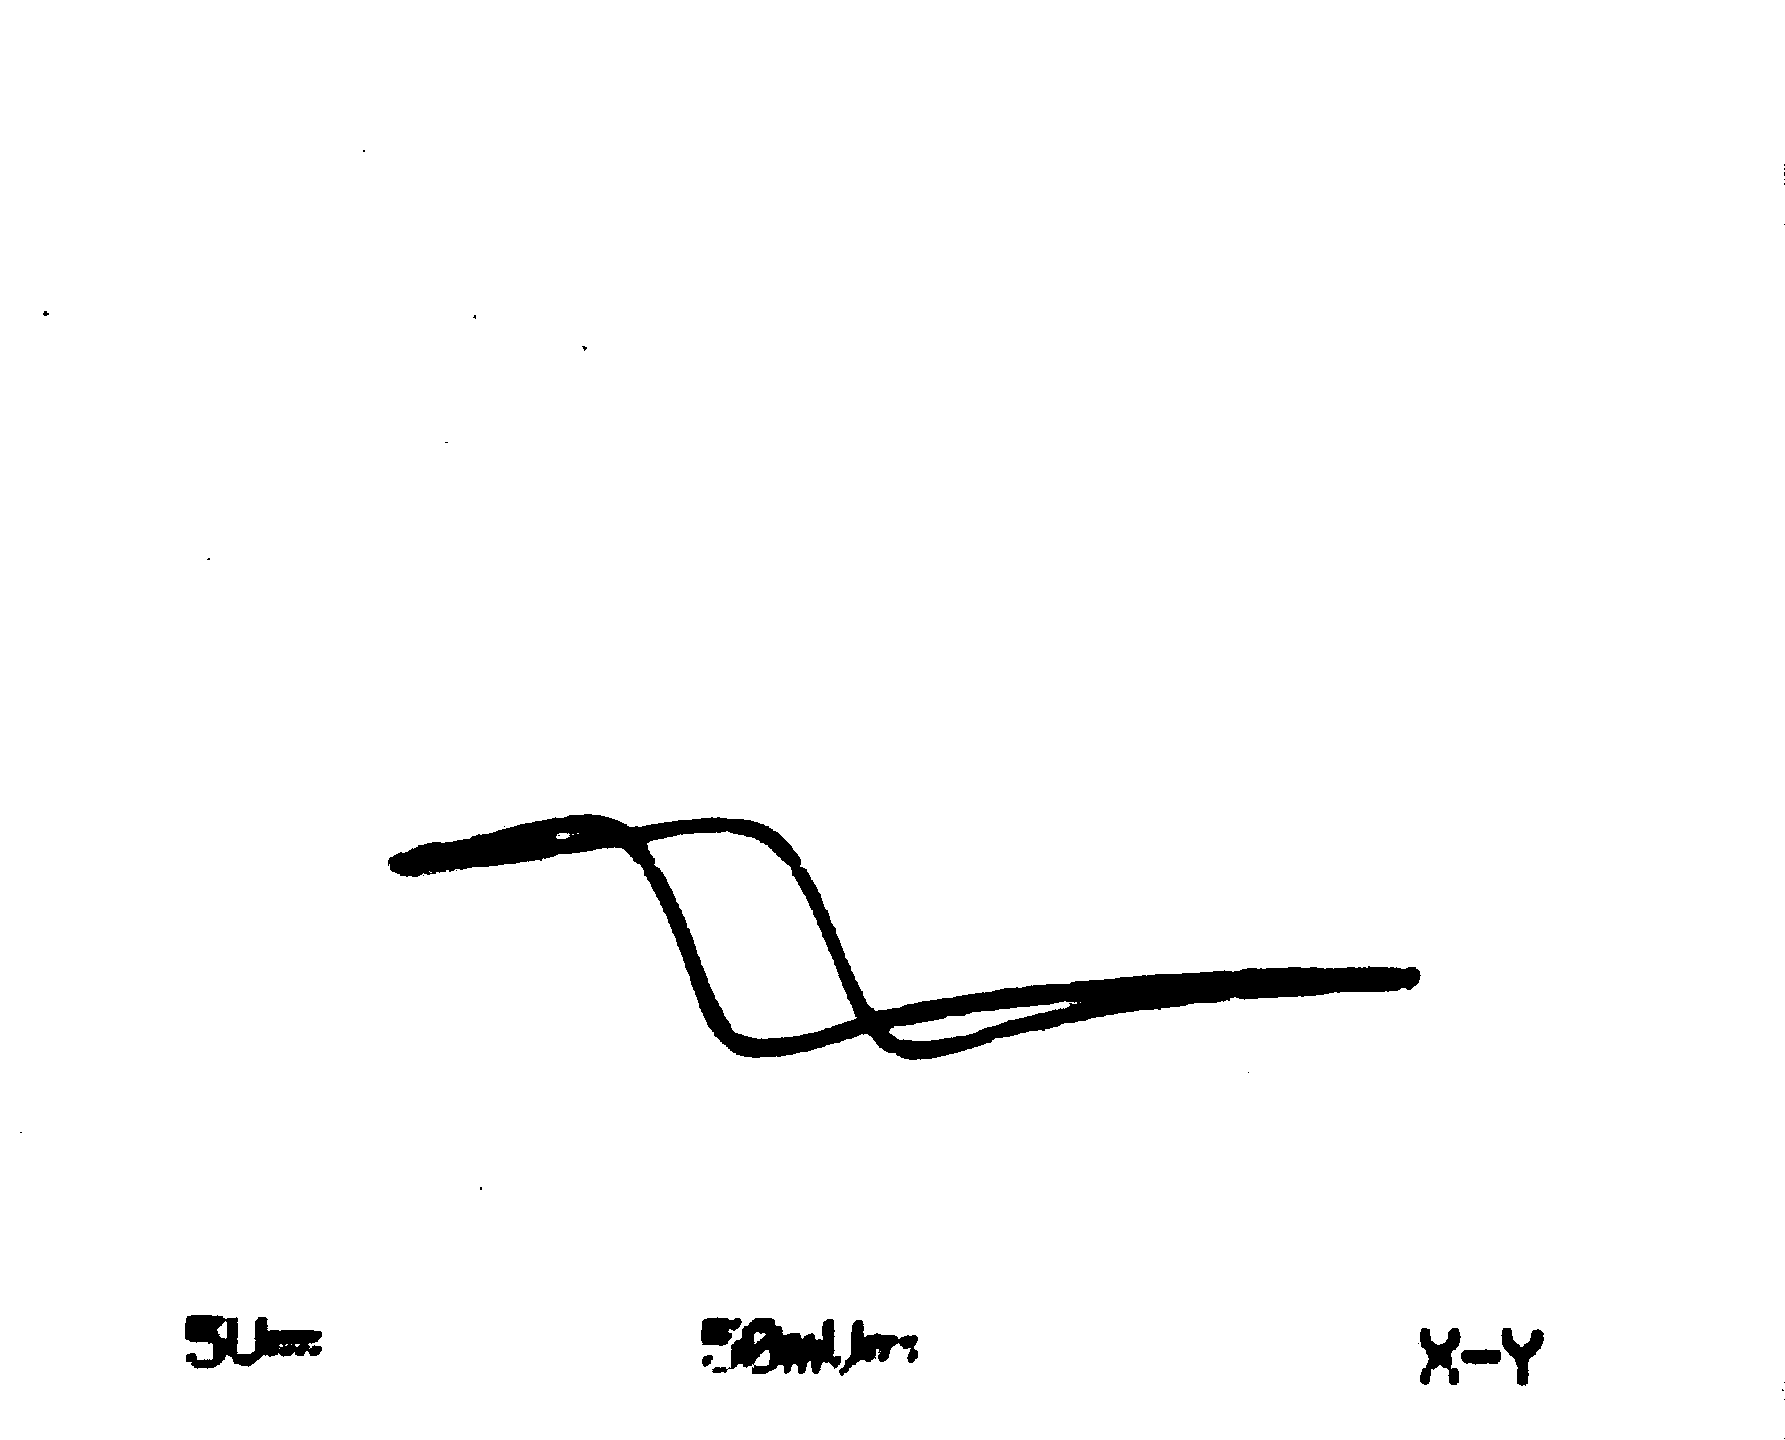
\includegraphics[height=4cm]{fig/oscilloscope/mma/wave4phasedev.png}\label{subfig:phasedev}}\hfill
		\subfloat[调节磁场之前]{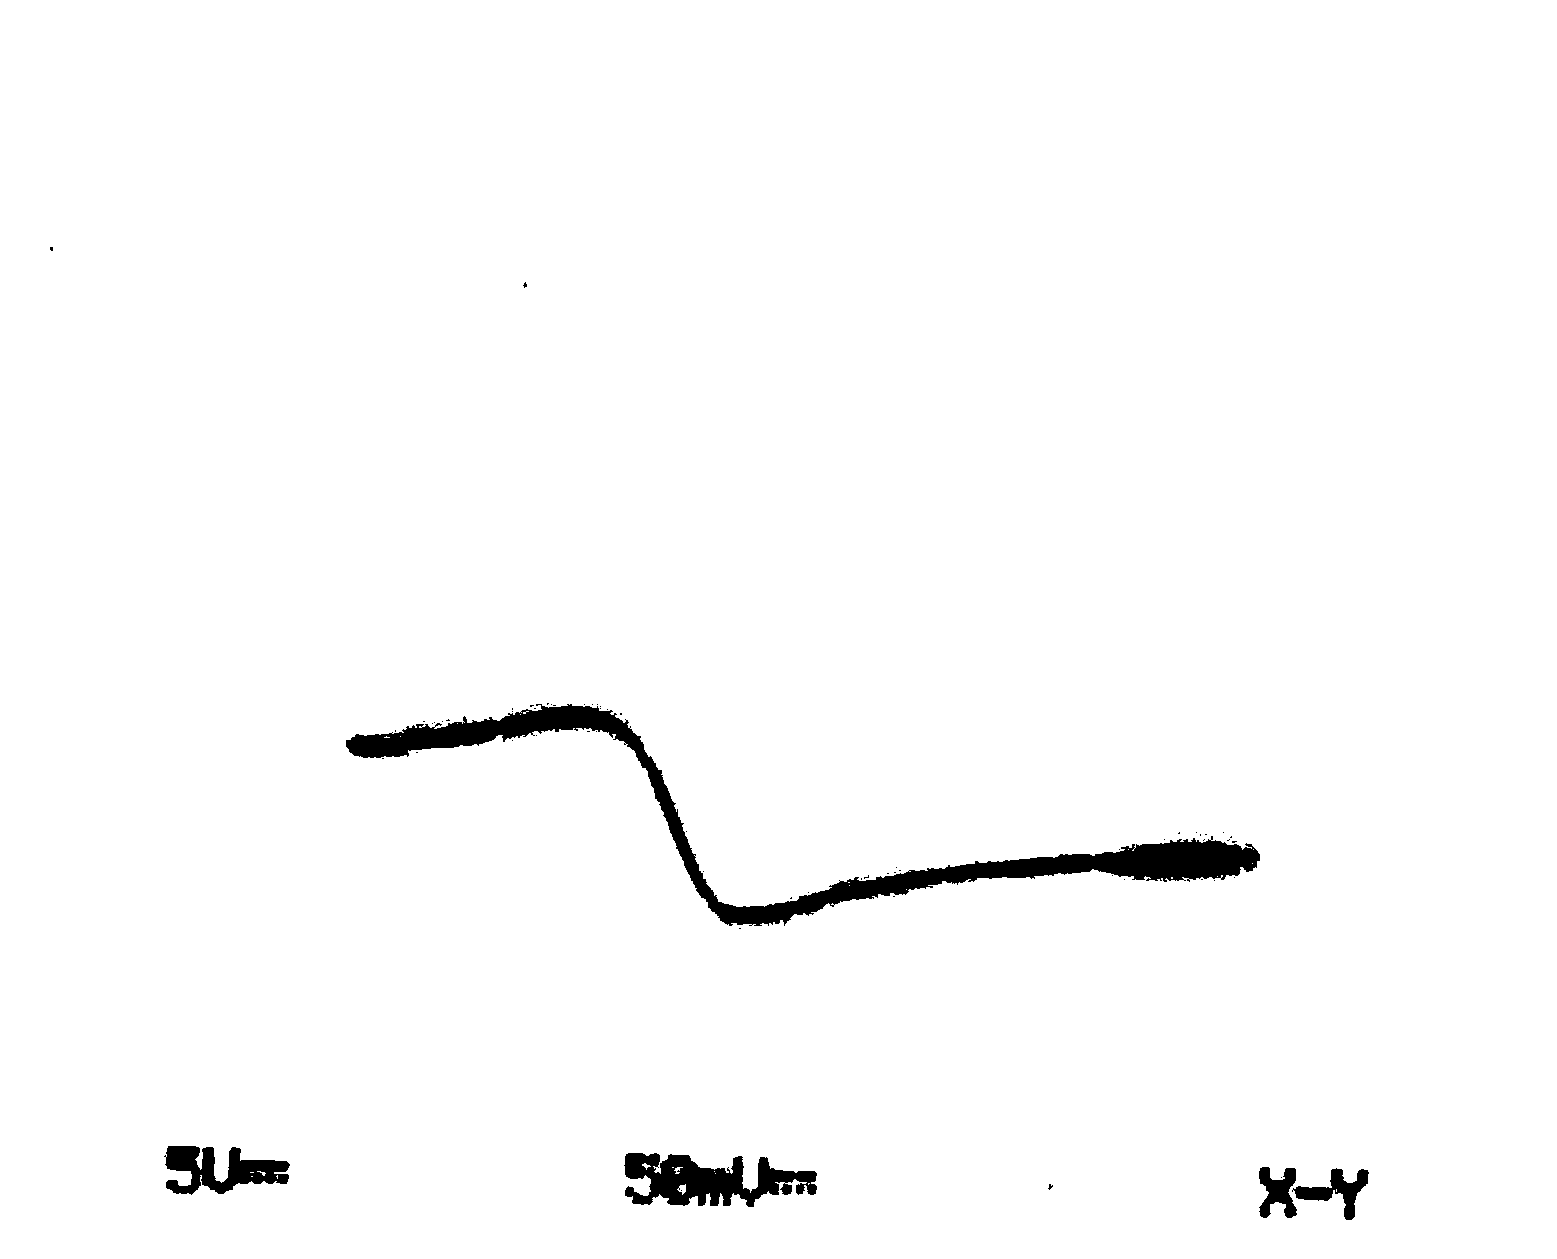
\includegraphics[height=4cm]{fig/oscilloscope/mma/wave5Bdiff.png}\label{subfig:Bdiff}}\hfill
		\subfloat[色散信号]{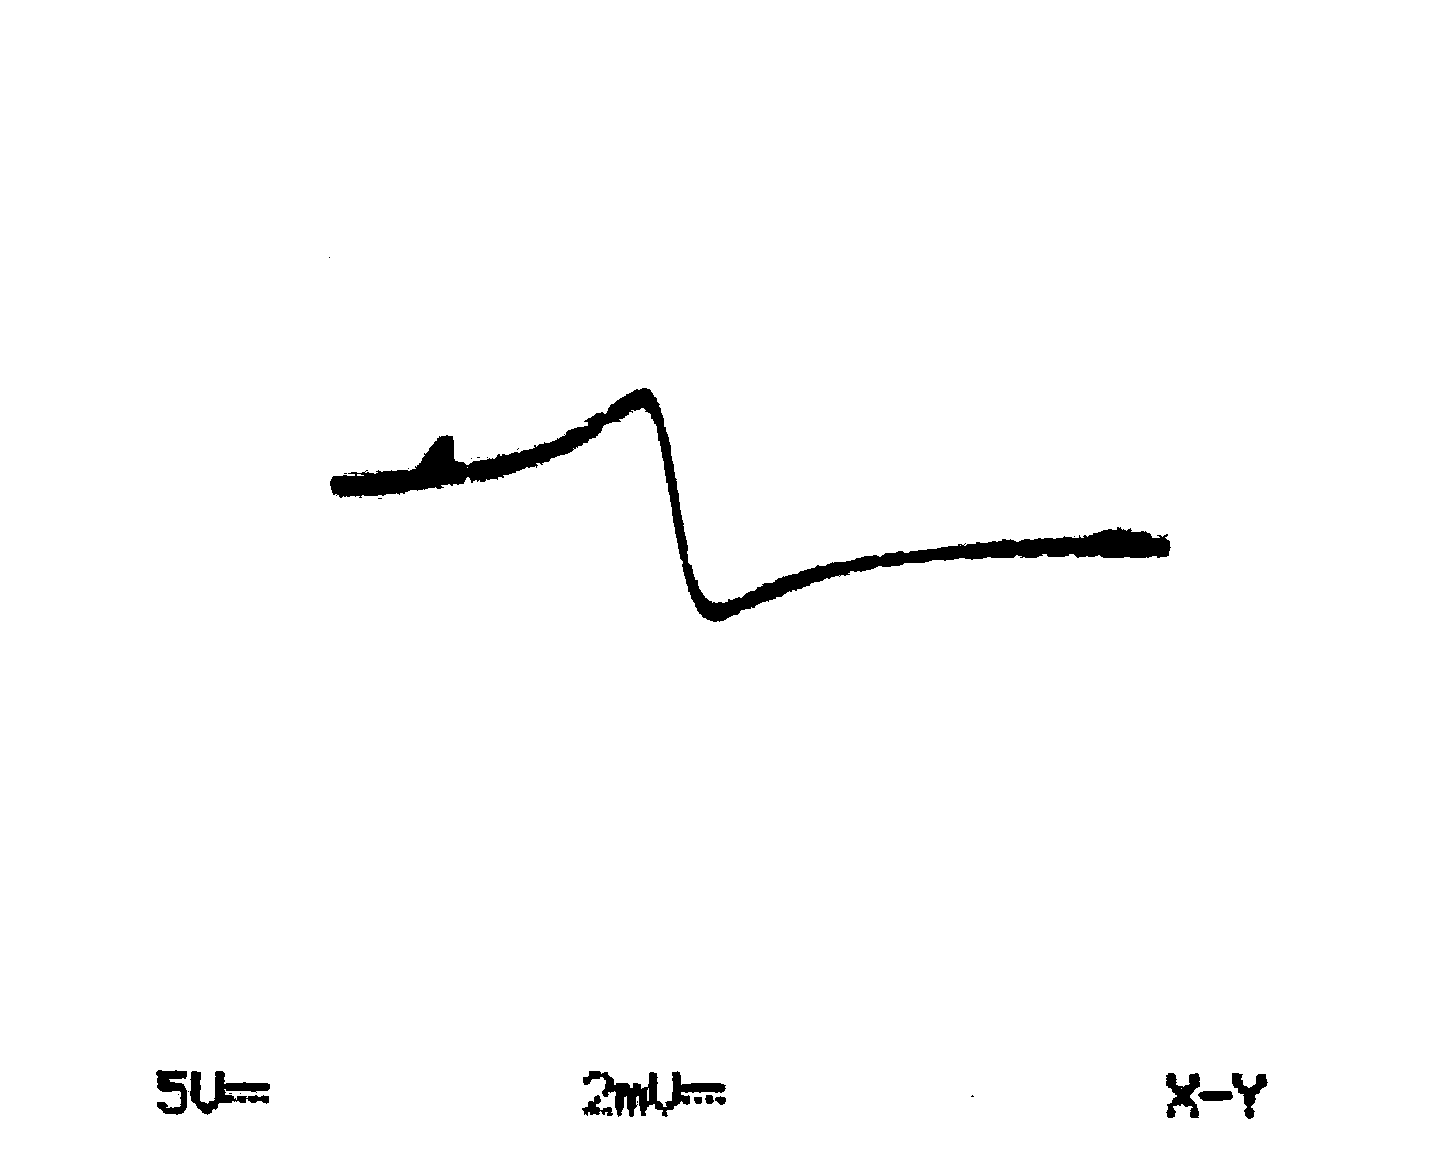
\includegraphics[height=4cm]{fig/oscilloscope/mma/wave6Bdiffu.png}\label{subfig:Bdiffu}}\\
		\subfloat[调节谐振频率前]{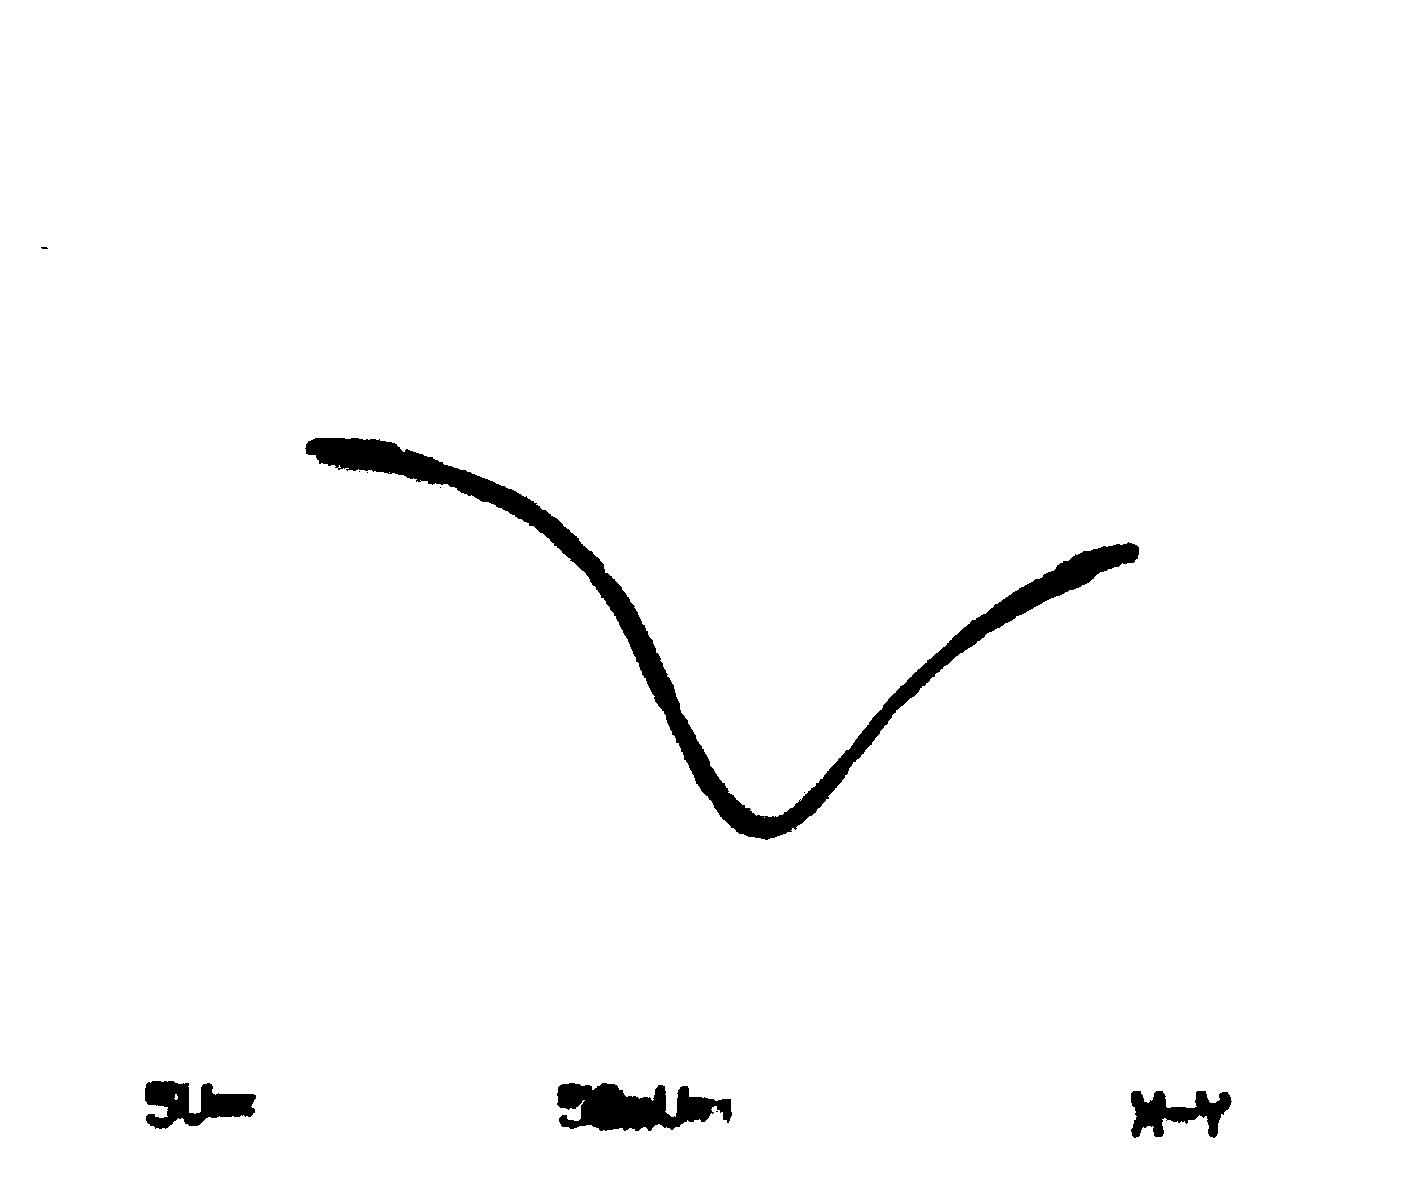
\includegraphics[height=4cm]{fig/oscilloscope/mma/wave8f0diff.png}\label{subfig:f0diff}}\hfill
		\subfloat[多晶样品]{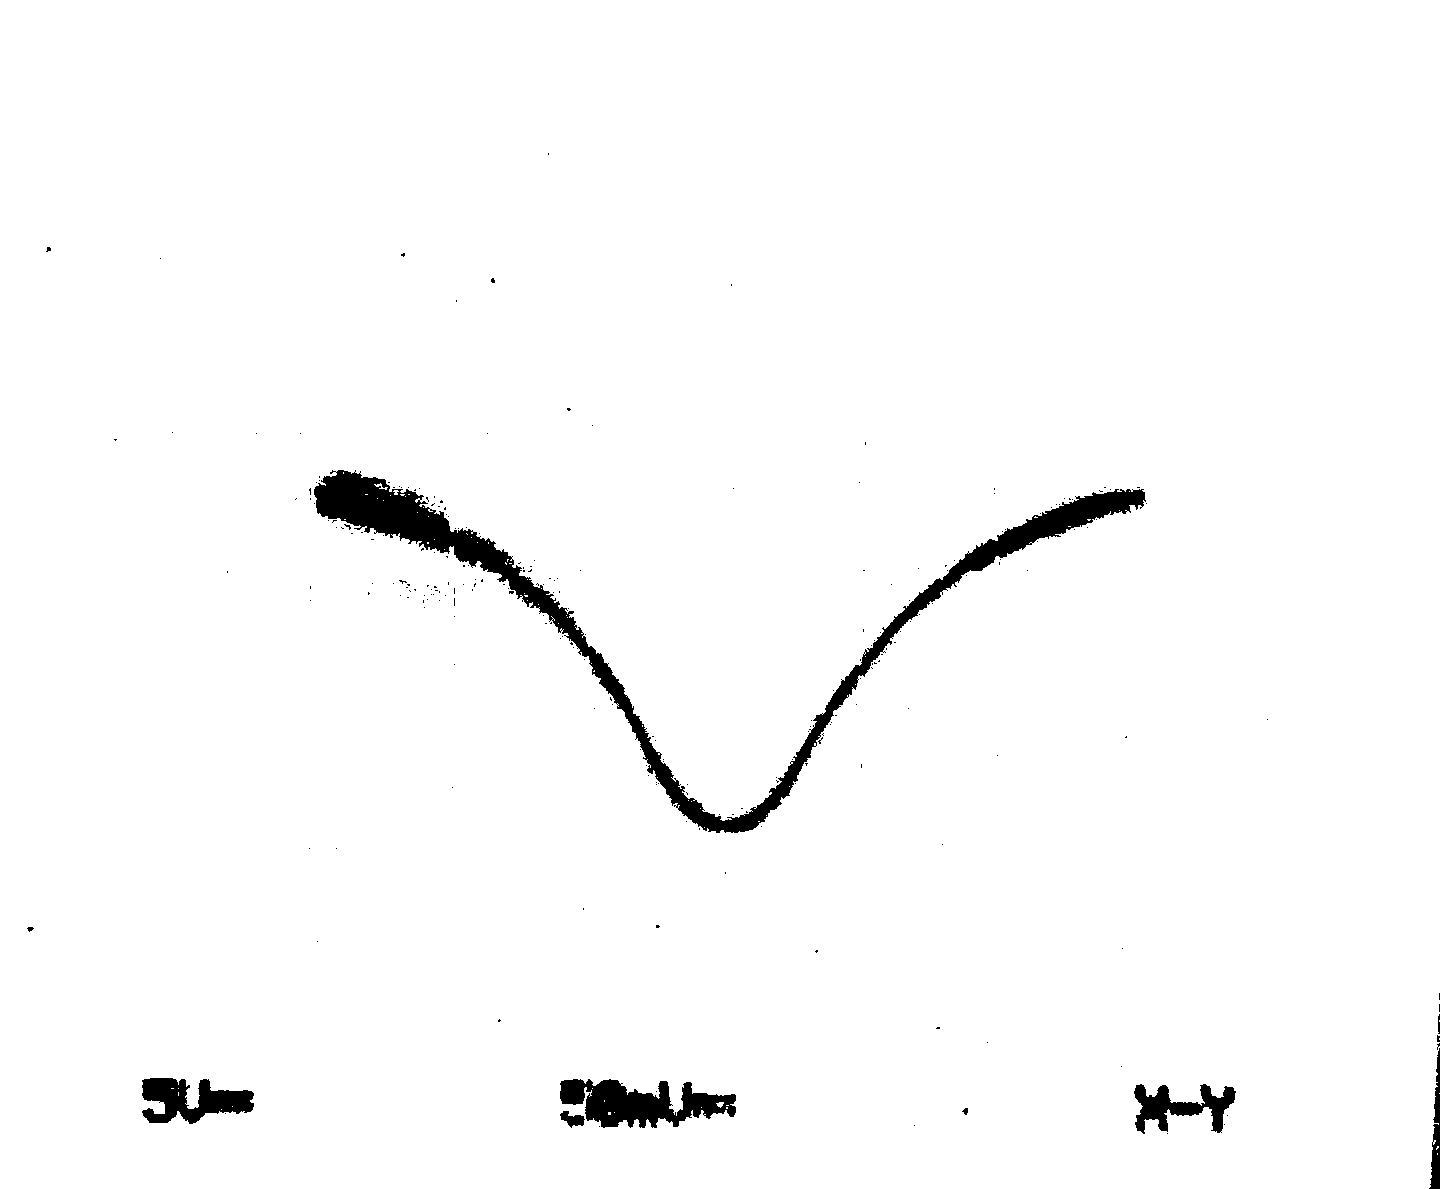
\includegraphics[height=4cm]{fig/oscilloscope/mma/wave9multiplecrystle.png}\label{subfig:multi}}\hfill
		\subfloat[单晶样品]{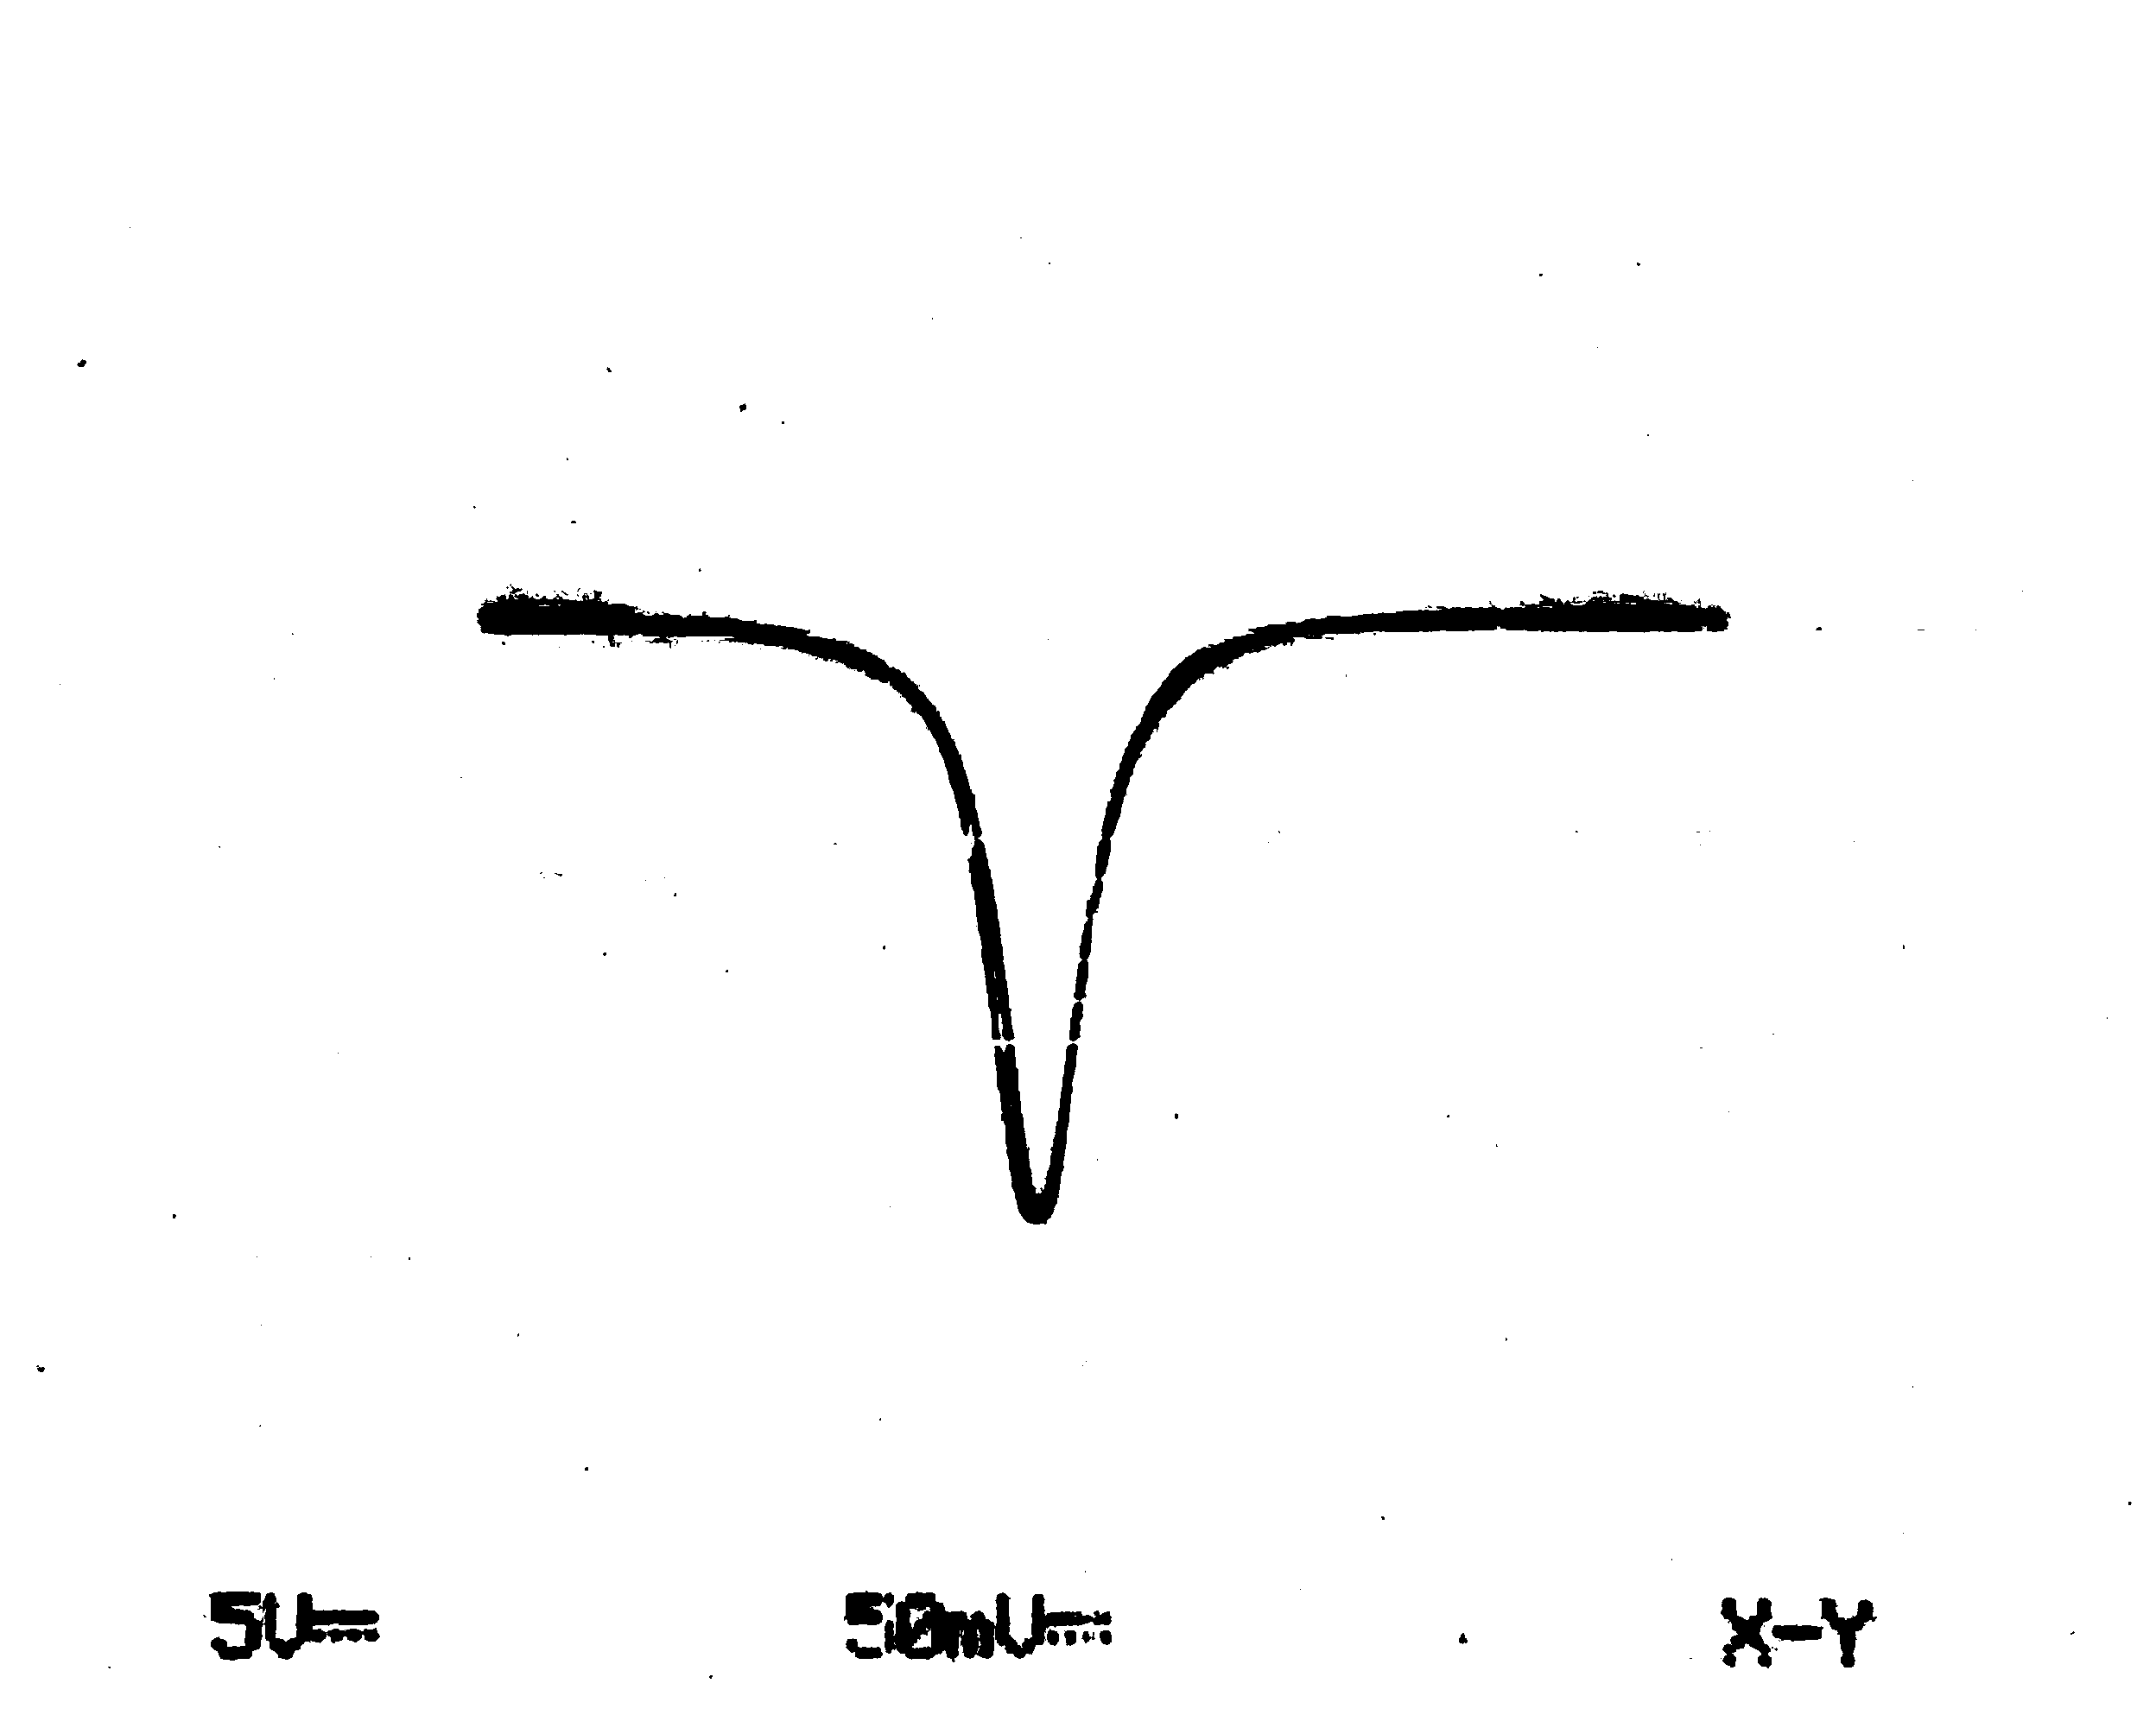
\includegraphics[height=4cm]{fig/oscilloscope/mma/wave10singlecrystle.png}\label{subfig:single}}
		\caption{示波器共振曲线}
	\end{figure}
	可见单晶铁氧体样品的共振线宽明显比多晶的更窄。这是因为多晶铁氧体可以看作是许多单晶组成的,组成它的单晶各自的谐振频率略有差异,叠加起来就体现为共振线宽更大的一个共振信号。
	% 在谐振腔中放入不同的铁氧体样品,观察共振信号的变化,记录共振曲线的图像,分析不同样品共振信号的差异与成因。
	\begin{figure}[htbp]
		\subfloat[多晶的铁磁共振图象逐点测量结果]{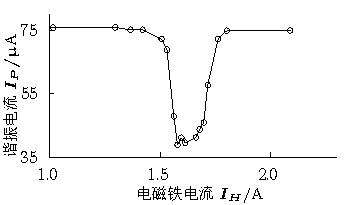
\includegraphics[height=4cm]{dat/prc/II.pdf}\label{subfig:II}}
		\subfloat[电磁铁定标曲线]{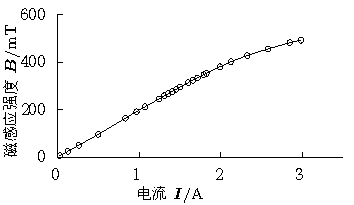
\includegraphics[height=4cm]{dat/prc/BI.pdf}\label{subfig:BI}}
		\caption{逐点法测量多晶样品的共振线宽}
	\end{figure}
	\begin{table}[htbp!]
	\centering\small
	\caption{谐振功率-磁场关系}\label{tab:II}	\begin{tabular}{c||c|c|c|c|c}
		\hline\hline
		电磁铁电流$I_{H}$/A & 谐振电流$I_{P}/\upmu$A & 谐振频率$f_0$/GHz & 电磁铁电流$I_{H}$/A & 谐振电流$I_{P}/\upmu$A & 谐振频率$f_0$/GHz\\		\hline\hline
		0.024 & 75.2 & 9.028 & 1.596 & 41.2 & 9.026\\		\hline
		1.015 & 75.9 & 9.026 & 1.614 & 39.6 & 9.027\\		\hline
		1.297 & 76 & 9.030 & 1.662 & 41.3 & 9.026\\		\hline
		1.366 & 75.2 & 9.028 & 1.679 & 43.8 & 9.026\\		\hline
		1.421 & 75.2 & 9.030 & 1.698 & 46 & 9.029\\		\hline
		1.507 & 72.3 & 9.027 & 1.716 & 57.8 & 9.029\\		\hline
		1.531 & 68.9 & 9.026 & 1.763 & 72.3 & 9.029\\		\hline
		1.562 & 48 & 9.031 & 1.802 & 74.9 & 9.026\\		\hline
		1.579 & 39 & 9.032 & 2.089 & 75 & 9.030\\		\hline\hline
	\end{tabular}
\end{table}
	\begin{table}[htbp!]
	\centering\small
	\caption{电磁铁磁场-电流定标}\label{tab:BI}	\begin{tabular}{c||c|c|c|c|c|c|c}
		\hline\hline
		电流$I$/A & {\tiny 磁感应强度}$B$/mT & 电流$I$/A & {\tiny 磁感应强度}$B$/mT & 电流$I$/A & {\tiny 磁感应强度}$B$/mT & 电流$I$/A & {\tiny 磁感应强度}$B$/mT\\		\hline\hline
		0.024 & 8 & 1.070 & 213 & 1.502 & 296 & 1.990 & 381\\		\hline
		0.123 & 26 & 1.242 & 246 & 1.601 & 314 & 2.126 & 402\\		\hline
		0.255 & 51 & 1.305 & 259 & 1.656 & 324 & 2.327 & 428\\		\hline
		0.495 & 97 & 1.356 & 268 & 1.714 & 334 & 2.580 & 456\\		\hline
		0.828 & 165 & 1.406 & 277 & 1.791 & 348 & 2.848 & 482\\		\hline
		0.963 & 192 & 1.450 & 286 & 1.825 & 353 & 2.986 & 493\\		\hline\hline
	\end{tabular}
\end{table}
	\par 为测量多晶样品的共振线宽$\Delta B$,将检波器2连接到微安表上,从小到大调节磁场电流,用逐点法测量其的共振曲线(谐振功率-磁场图象);结果如\cref{subfig:II,tab:II}所示。其中每次测量前都已重新将谐振腔调谐。测得远离谐振位置的功率指示电流约为$I_{P,0}=75.4\upmu$A(这是功率指示电流稳定部分的几个数据点的均值),谐振位置的功率指示电流为$I_{P,0}=39\upmu$A。于是根据\cref{eq:p}可以求出$I_{P,\frac{1}{2}}=52.8\upmu$A。经线性插值可得这一功率对应的电磁铁电流为1.5549A和1.7084A。于是得到多晶样品的共振线宽(以电磁铁电流表示)为$\Delta I_{H}\approx 0.15345$A。
	\par 用高斯计标定电磁铁电流与磁场强度的关系如\cref{subfig:BI,tab:BI}所示。经线性插值得到上述两个电流1.5549A和1.7084A对应的磁感应强度分别约为305.62mT和333.03mT;所以共振线宽为
	\begin{equation}
		\Delta B=27.41{\rm mT}.
	\end{equation}
	\par 同样地可以插值得出谐振位置的磁感应强度为$B_0\approx 310.00$mT。由此可以计算样品的旋磁比
	\begin{equation}
		\gamma =\dfrac{\omega_0}{B_0}=1.831\times 10^{5}{\rm T}\cdot{\rm s}.
	\end{equation}
	由此求出$g$因子为
	\begin{equation}
		g=\dfrac{2m\gamma}{\mu_0 e}=1.655.
	\end{equation}
	弛豫时间为
	\begin{equation}
		\tau = \dfrac{2}{\gamma \Delta H}=1.586\times 10^{-4}{\rm s}.
	\end{equation}
	\par 单晶样品由于谐振范围过窄,仪器分辨率难以测出共振线宽。
	\par 在示波器图象中可见多晶样品的共振线宽较大,故其弛豫时间较短。这是因为多晶中的磁畴的$M_{S}$较小,更易受外磁场影响偏转。
% subsubsection 铁磁共振实验 (end)
%	\item 关机:将铁磁共振仪的电磁铁电流调至最小,关仪器电源开关。